\section{Vývoj projektu}

V~této sekci jsou popsány technologie využité při vývoji portálu \bso{} a důvody pro jejich výběr, postup vývoje projektu a získané zkušenosti s vývojem i samotným provozem.

\subsection{Využité technologie}
\label{sub:used-technologies}

Při vývoji projektu byl využit programovací jazyk \nameref{sub:php} s~\gls{framework}em  \nameref{subsub:laravel}. Pro \gls{real-time} funkcionality, jako chat a notifikace, byl využit \gls{open-source} implementace aplikace \nameref{subsub:pusher}, Laravel Websockets\cite{laravel-websockets}. Jako \acrshort{rdbms} jsem využil MySQL\cite{mysql}. Emailové služby pro aplikaci zajišťuje služba Amazon SES\cite{amazon-ses}.

\subsubsection{PHP a Laravel}

Jelikož byla na začátku projektu \bso{} klíčová rychlost dodání \gls{mvp} byl vybrán jazyk \nameref{sub:php} společně s~\gls{framework}em \nameref{subsub:laravel} z~důvodu jednoduchosti nasazení, nízkých nákladů na provoz a velké flexibility a rychlosti vývoje. Dalším velkým plus jsou pomocné utility jako Composer\cite{composer} nebo Laravel Artisan Console\cite{laravel-artisan} a rozšíření Laravel Idea\cite{laravel-idea} pro \acrshort{ide} PhpStorm\cite{phpstorm}.

Laravel, skrze Laravel Jetstream\cite{laravel-jetstream}, poskytuje předpřipravené části aplikace jako registrace a ověřování uživatelů, \acrshort{css} \gls{framework} Tailwind CSS\cite{tailwind-css} a JavaScriptový \gls{scaffolding} Inertia.js\cite{inertia-js} nebo Laravel Livewire\cite{laravel-livewire}.

\begin{figure}[h]
\centering
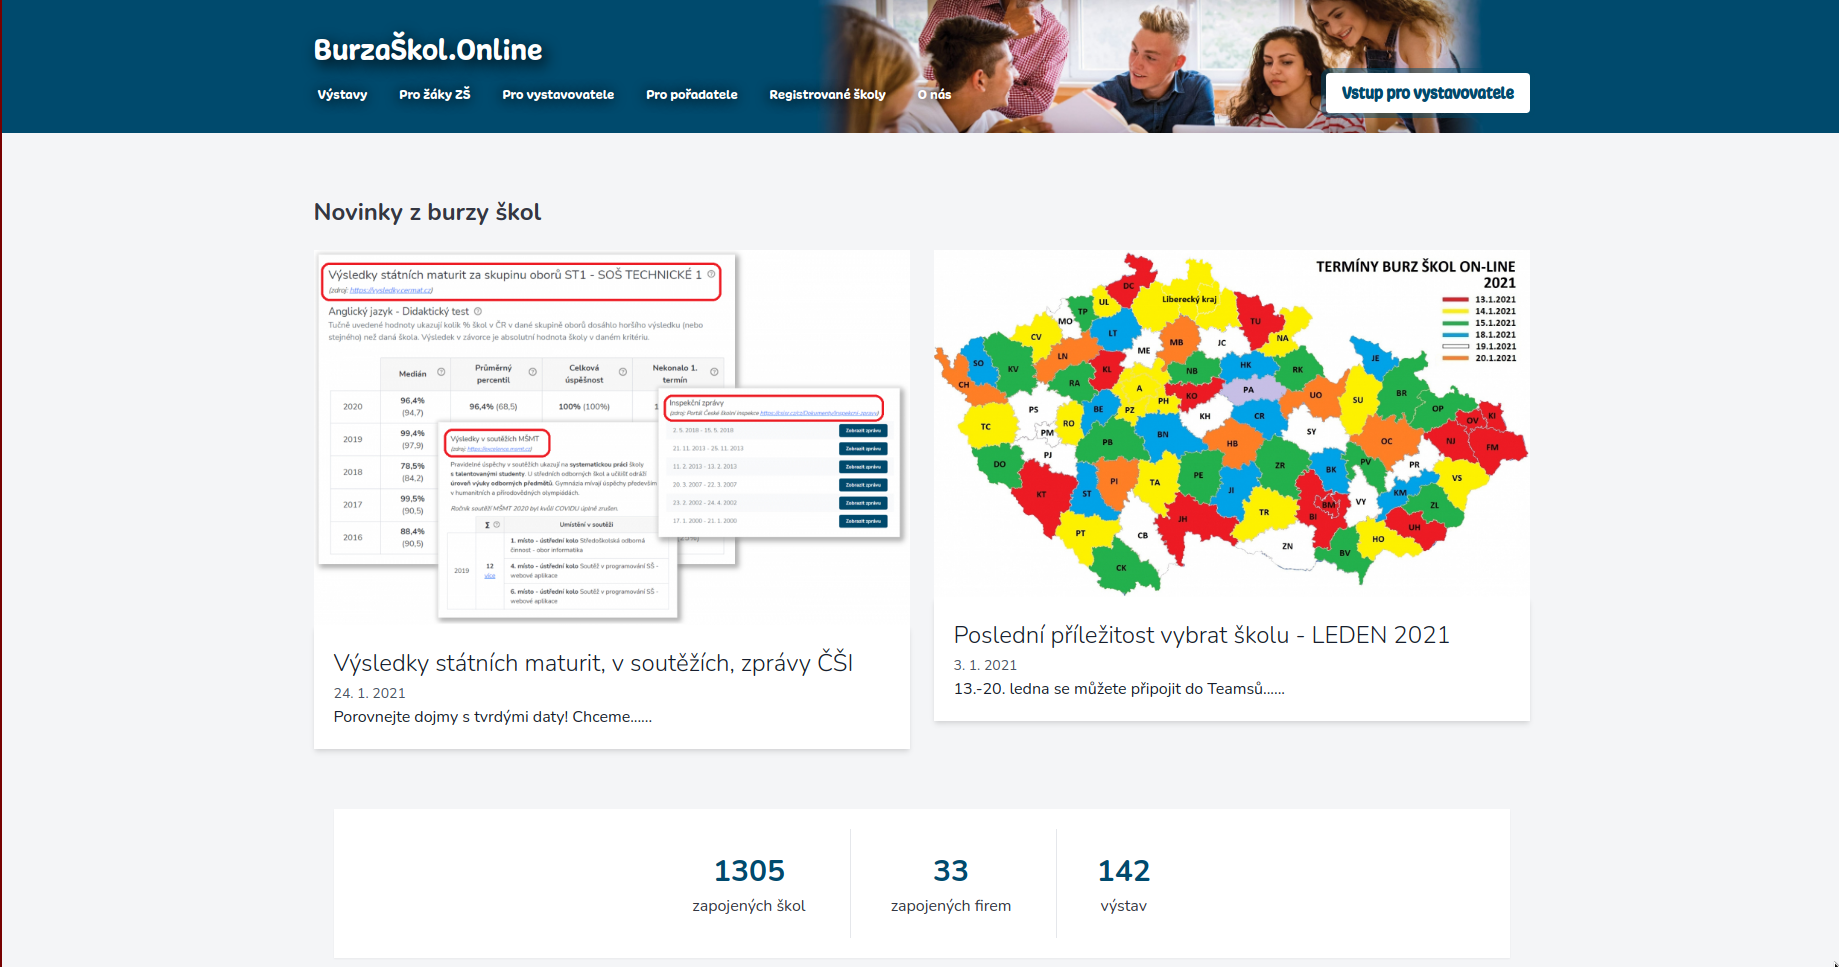
\includegraphics[width=\textwidth]{img/burzaskol-online.png}
\caption{Aplikace \bso{}}
\label{fig:burzaskol-online-2020}
\end{figure}

\subsubsection{Pusher}

Technologii Pusher byla vybrána z~důvodu jednoduché integrace do stávajícího projektu a možnosti pokročilého ladění. Z~implementačních důvodů byla využita \gls{open-source} implementace protokolu Pusher nazvaná \uv{Laravel Websockets}. To nám poskytlo větší kontrolu nad nasazením a škálováním projektu.

\subsubsection{MySQL}

\acrshort{rdbms} MySQL oproti ostatním relačním databázím vyniká jednoduchostí správy a množstvím poskytovatelů spravovaných databázových instancí\cite{mysql-vs-others}.
Výše uvedené, a excelentní integrace s~jazykem \acrshort{php} a \gls{framework}em Laravel, z~ní dělá ideální volbu pro vývoj webových aplikací.
Velkým přínosem je také široká řada nástrojů jako mysqldump\cite{mysqldump} nebo phpMyAdmin\cite{phpmyadmin}, které významně zjednodušují správu a provoz databáze MySQL.

\subsubsection{Amazon SES}

\acrfull{aws} poskytuje v~rámci služby \acrfull{aws-ses} jednoduchou a cenově dostupnou emailovou bránu. Ta nabízí funkcionality jako \gls{dkim} podepisování emailů a zobrazování pokročilých statistik jako počet odeslaných emailů, počet \uv{odražených} emailů\cite{email-bounce} a počet stížností na námi zaslanou poštu.

\subsection{Přípravy na vývoj projektu}

Předtím než může započít vývoj \acrshort{sw} projektu je zapotřebí se zadavatelem vytvořit zadání.
Jedná se o~dokument popisující jednotlivé konkrétní funkcionality a procesy aplikace. 
Ze zadání by měly vycházet veškeré části aplikace jako je datový model a použité technologie.
\emph{Zadání by mělo být konkrétní a jednoznačné, pokud existuje více výkladů, může dojít k~velkým problémům při vývoji aplikace.} 

Dalším krokem je výběr technologií, které budou na vývoj projektu použity.
Ze zadání určíme pro jakou platformu bude projektu určen, zda-li se jedná o~webovou, desktopovou, mobilní, serverovou nebo kombinovanou aplikaci.
Dle toho vybereme konkrétní technologie jako např Laravel\cite{laravel} pro vývoj aplikace, MySQL\cite{mysql} pro ukládání dat a Git\cite{git} pro správu zdrojového kódu.

Když jsou zvoleny technologie, můžeme začít vytvářet datový model pro vybraný typ databáze.
Dále rozvrhneme jednotlivé obrazovky a postupy, které bude aplikace obsahovat.
Je také potřeba vytvořit plán nasazení projektu, tedy jak bude aplikace hostováná, či jaký mail server využijeme.

Když máme všechny přípravy hotovy, můžeme přejít k~samotnému programování projektu.

\subsection{Vývoj projektu ve frameworku Laravel}
\label{sub:laravel-development}

Prvním krokem při vývoji projektu \inlaravel, je vytvoření tříd tzv. \emph{modelů}\cite{laravel-models} a k~nim náležejících \emph{migrací}\cite{laravel-migrations}. Ty vytvoříme dle připraveného datového modelu.

Když jsou modely a migrace úspěšně vytvořeny můžeme přistoupit k~vytváření \emph{kontrolerů}\cite{laravel-controller}, \emph{komponent}\cite{laravel-blade-component} a definování \emph{cest}\cite{laravel-routes}.

\subsubsection{Modely}

Modely jsou \acrshort{php} třídy reprezentující samostatné databázové tabulky, řádky a relace mezi nimi. Modely nám dovolují vytvářet, upravovat a filtrovat záznamy jako by se jednalo o~nativní \acrshort{php} objekty. To velice zjednodušuje práci s~daty.

V~současné době aplikace \bso{} obsahuje 26 modelů, např. \emph{School} pro vystavovatele nebo \emph{Region} pro kraj. 

\subsubsection{Migrace}

Migrace, \inlaravel, slouží pro kontrolované úpravy databáze. Jejich hlavní úkol je udržet databázi v~konzistentním stavu s~verzí aplikace. Při nasazení nové verze tedy stačí spustit migrace a databáze je synchronizována s~verzí aplikace.

\subsubsection{HTTP cesty}

\acrshort{http} cesty definují jaký kód je spuštěn při \acrshort{http} požadavku. Cesta je identifikována pomocí jedné, či více \acrshort{http} metod a \acrshort{http} cesty. Cesta v~sobě může obsahovat parametry, např. id knihy. Cesta může vést na \emph{\acrshort{http} přesměrování}, \emph{\acrshort{php} funkci} nebo \emph{\acrshort{http} kontroler}.

Aplikace \bso{} definuje 38 unikátních \acrshort{http} cest. Velké množství \acrshort{http} cest dále přijmá různé parametry, které dále ovlivňují obsah vygenerované stránky.

\subsubsection{HTTP kontrolery}

\acrshort{http} kontrolery, \inlaravel, jsou \acrshort{php} třídy obsahující \expl{logiku pro zpracování \acrshort{http} cest}{handlery, \acrshort{php} metody}. Můžeme je rozdělit na standardní kontrolery, \emph{single-action kontrolery}\cite{laravel-controller-single-action} a \emph{resource kontrolery}\cite{laravel-controller-resource}.

Standardní kontrolery obsahují libovolný počet handlerů. Při definování \acrshort{http} cesty musíme definovat jak kontroler, tak metodu, která má být zavolána.

Single-action kontrolery obsahují pouze metodu \emph{\_\_invoke}. Jsou vhodné pokud je logika pro nějakou cestu velice komplexní a je lepší ji izolovat. Při definování cesty stačí zmínit pouze název třídy a \nameref{subsub:laravel} metodu automaticky spáruje.

Resource kontrolery mají přesně definovanou strukturu. Obsahují skupinu metod pro vytváření, úpravu a čtení daného \expl{zdroje}{resource}. Cesty se definují skupinově pomocí statické metody \emph{resource}.

\subsubsection{Blade komponenty}

Všechny aplikace mají za cíl zobrazovat uživateli informace. Webové aplikace využívají k~zobrazování informací značkovací jazyk \acrshort{html}.

U~jednoduchý stránek můžeme využít statických \acrshort{html} souborů, které jsou pro každý požadavek stejné a nemění se. Pro úpravu obsahu stránky je nutný přístup k~hostingové službě a znalost \acrshort{html}.

Moderní webové aplikace vyžadují obsah dynamický, který je závislý na velké řadě faktorů, např. zda-li je uživatel přihlášen, jaká jsou jeho oprávnění, či jaké výstavy se právě konají. Obsah těchto stránek je většinou uživatelsky editovatelný za pomocí grafického \acrshort{wysiwyg} editoru.

Pro generování těchto stránek se používají šablonovací nástroje jako samotné \acrshort{php} nebo různé pomocné knihovny jako Twig\cite{twig} nebo Laravel Blade Views\cite{laravel-blade}. Takové knihovny nám dovolují psát čisté \acrshort{html} s~přídavkem speciálních příkazů. Tyto příkazy nám dovolují například podmínečné generování, možnost vypisovat a formátovat \acrshort{php} proměnné nebo modularizaci stránek na menší znovupoužitelné komponenty.
